\documentclass[../main.tex]{subfiles}
\begin{document}
For the string problems, it can be divided into two categories: \textbf{one string} and \textbf{two strings pattern matching}. 

For the one string problem, the first type is to do operations that meet certain requirements on a single string. (1). For the ad hoc easy string processing problems, we only need to read the requirement carefully and use basic programming skills, data structures, and sometimes requires us to be farmilar with some string libraries like Re other than the basic built-in string functions. We list some LeetCode Problems of this type in Section~\ref{string_ad_hoc}. (2) There are also more challenging problems: including find the longest/shortest/ count substring and subsequence that satisfy certain requirements. Usually the subsequence is more difficult than the substring. In this chapter we would list the following types in Section~\ref{string_advanced_single}
\begin{itemize}
    \item Palindrome: A sequence of characters read the same forward and backward.
    \item Anagram: A word or phrase formed by rearranging the letters of a different word or phrase.
    \item Parentheses and others. 
\end{itemize}


\textbf{Application for Pattern Matching for two strings:} Given two strings or two arrays, one is S, and the pattern P, The problems can be generalized to find pattern P in a string S, you would be given two strings. (1) If we do not care the order of the letters (anagram) in the pattern, then it is the best to use Sliding Window; This is detailed in Section~\ref{string_anagram} (2) If we care the order matters (identical to pattern), we use KMP. The problems of this type is listed in Section~\ref{string_exact_matching}.

% \textbf{Brute Force Exact Pattern Matching} Before we proceed to the efficient pattern matching algorithms, let us take a look at how we do the pattern matching with brute force. Assume we are given a string S and a pattern P, now we need to search the position of P in S, if we do not use the built-in functions in Python, what would we do to solve this problem.

% Solution: it is straightforward that we need to compare S and P char by char. Suppose now we are matching the ith char of  S to the jth char in the P, all the previous j-1 chars in P have already been matched in S. Now we would have two situations: if S[i] == P[j], then we move forward i and j to the next position, otherwise, the match failed, for example S="ABCDF" and P="ABCE", when the i=3, and j = 3, 'D'!='E', so that j need to move to position j=0, which has backtracked j positions, and for the S, we need to move to char 'B', which only backtrack j-1 positions, so that $i - i_{new} = j-1$, which makes $i_{new} = i-j+1$. The Python code of the brute force solution is:
% \begin{lstlisting}[language = Python]
% def bruteForcePatternMatching(S, P):
%     sLen, pLen = len(S), len(P)
%     i, j = 0, 0
%     while i < sLen and j < pLen:
%         if S[i] == P[j]:
%             i += 1
%             j += 1
%         else:
%             i = i -j + 1
%             j = 0
            
%     if j == pLen:
%         return i - j
%     else:
%         return -1 
% \end{lstlisting}
% This can only return the first match, to modify it that we can find all patterns in the string, we can do as follows: 
% \begin{lstlisting}[language = Python]
% def bruteForcePatternMatchingAll(S, P):
%     if not S or not P:
%         return []
%     sLen, pLen = len(S), len(P)
%     i, j = 0, 0
%     ans = []
%     while i < sLen:
%         if j == pLen: #collect position
%             ans.append(i - j)
%             j = 0
%             i = i -j + 1
%             continue
%         # do the pattern matching  
%         if S[i] == P[j]:
%             i += 1
%             j += 1
%         else:
%             i = i -j + 1
%             j = 0
%     return ans
% \end{lstlisting}
% The time complexity for brute force pattern matching is $O(S*P)$. It is not hard to see that when one char does not match, with the backtracking, we backtrack j-1 positions in S, and j positions in P. For example, S = "ABCDABD ABCDABCDABDE", P = "ABCDABD", when P match "ABCDABC" at the second 'C', then if we know .... With KMP, we can make the worst case time complexity to be $O(S)$.
% \section{Word Subsets}
\section{Ad Hoc Single String Problems}
\label{string_ad_hoc}
\begin{enumerate}
    \item 125. Valid Palindrome
    \item 65. Valid Number
    \item 20. Valid Parentheses (use a stack to save left parenthe)
    \item 214. Shortest Palindrome (KMP lookup table)
    \item 5. Longest Palindromic Substring
    \item 214 Shortest Palindrome , KMP lookup table, for example s=abba, constructed S = abba\#abba),
    \item 58. Length of Last Word(easy)
\end{enumerate}

\section{String Expression}
\begin{enumerate}
    \item 8. String to Integer (atoi) (medium)
\end{enumerate}
%%%%%%%%%%%Advanced slingle string%%%%%%%%%%%%%%%%%%%%%%%%%%
\section{Advanced Single String}
\label{string_advanced_single}
    For hard problem, reconstruct the problem to another so that it can be resolved by an algorithm that you know.
%%%%%%%%%%%%%%%%% palindrome %%%%%%%%%%%%%%%%%%%%%%%%%%%%%%%%%%%%%
\subsection{Palindrome}
Palindrome is a sequence of characters read the same forward and backward. To identify if a sequence is a palindrome say ``abba" we just need to check if s == s[::-1]. In the structure, if we know ``bb" is palindrome, then ``abba" should be palindrome if s[0] == s[3]. Due to this structure, in the problems with finding palindromic substrings, we can apply dynamic programming and other algorithms to fight back the naive solution. 

To validate a palindrome we can use two pointers, one at the start, and the other and the end. We iterative them into the middle location. 
\begin{enumerate}

    \item 409. Longest Palindrome (*)
    \item 	9. Palindrome Number (*)
    \item 	Palindrome Linked List (234, *)
    \item Valid Palindrome (125, *)
    \item Valid Palindrome II   (680, *)
    \item Largest Palindrome Product (479, *)
    \item 647. Palindromic Substrings (medium, check)
    \item Longest Palindromic Substring (5, **, check)
    \item Longest Palindromic Subsequence(516, **)
    \item Shortest Palindrome  (214, ***)
    \item Find the Closest Palindrome(564, ***)
    \item Count Different Palindromic Subsequences(730, ***)
    \item Palindrome Partitioning (131, **)
    \item Palindrome Partitioning II (132, ***)

    \item 266. Palindrome Permutation (Easy)
    \item Palindrome Permutation II  (267, **)
    \item Prime Palindrome (866, **)
    \item Super Palindromes (906, ***)
    \item Palindrome Pairs (336, ***)
    \item 
\end{enumerate}
\begin{examples}[resume]
\item \textbf{Valid Palindrome II (L680, *).} Given a non-empty string s, you may delete \textbf{at most} one character. Judge whether you can make it a palindrome. 
\begin{lstlisting}[numbers=none]
Example 1:

Input: "aba"
Output: True

Example 2:

Input: "abca"
Output: True
Explanation: You could delete the character 'c'.
\end{lstlisting}
\textbf{Solution: Two Pointers.} If we allow zero deletion, then it is a normal two pointers algorithm to check if the start i and the end j position has the same char. If we allow another time deletion is when the start and end char is not equal, we check if deleting s[i] or s[j], left s(i+1, j) or s(i, j-1) if they are palindrome. 
\begin{lstlisting}[language=Python]
def validPalindrome(self, s):
    if not s:
        return True
    
    i, j = 0, len(s)-1
    while i <= j:
        if s[i] == s[j]:
            i += 1
            j -= 1
        else:
            left = s[i+1: j+1]
            right = s[i:j]
            return left == left[::-1] or right == right[::-1]
    return True
\end{lstlisting}
\item \label{l647} \textbf{Palindromic Substrings(L647, **).}  Given a string, your task is to count how many palindromic substrings in this string. The substrings with different start indexes or end indexes are counted as different substrings even they consist of same characters. 
\begin{lstlisting}[numbers=none]
Example 1:

Input: "abc"
Output: 3
Explanation: Three palindromic strings: "a", "b", "c".

Example 2:

Input: "aaa"
Output: 6
Explanation: Six palindromic strings: "a", "a", "a", "aa", "aa", "aaa".
\end{lstlisting}
\textbf{Solution 1: Dynamic Programming.} First, we use dp[i][j] to denotes if the substring s[i:j] is a palindrome or not. Thus, we have a matrix of size $n\times n$. We an apply a simple example ``aaa".
\begin{lstlisting}[numbers=none]
``aaa"
    0  1  2
0   1  1  1
1   0  1  1
2   0  0  1
\end{lstlisting}
From the example, first, we know this matrix would only have valid value at the upper part due to i<=j. Because if j-i>=3 which means the length is larger or equals to 3, dp[i][j] = 1 if s[i]==s[j] and dp[i+1][j-1]==1. Compare i:i+1, j:j-1. This means we need to iterate i reversely and j incrementally.
\begin{lstlisting}[language=Python]
def countSubstrings(self, s):
    """
    :type s: str
    :rtype: int
    """
    n =len(s)
    dp = [[0 for _ in range(n)] for _ in range(n)] # if from i to j is a palindrome
    res = 0
    for i in range(n-1,-1,-1):
        for j in range(i,n):                
            if j-i>2: #length >=3
                dp[i][j] = (s[i]==s[j] and dp[i+1][j-1])
            else:
                dp[i][j] = (s[i]==s[j]) #length 1 and 2
            if dp[i][j]:
                res += 1
    return res
\end{lstlisting}
\textbf{Range Type Dynamic Programming.}A sligtly different way to fill out the matrix is:
\begin{lstlisting}
def countSubstrings(self, s):
    if not s:
        return 0
    
    rows = len(s)
    dp = [[0 for col in range(rows)] for row in range(rows)]
    ans = 0
    for i in range(0,rows):
        dp[i][i] = 1
        ans += 1
    
    for l in range(2, rows+1): #length of substring
        for i in range(0,rows-l+1): #start 0, end len -l+1
            j = i+l-1
            if j > rows:
                continue
            if s[i] == s[j]:
                if j-i > 2:
                    dp[i][j] = dp[i+1][j-1]
                else:
                    dp[i][j] = 1
            ans += dp[i][j]
                
    return ans
\end{lstlisting}
\textbf{Solution 2: Center Expansion.} For s[0]='a', it is center at 0, s[0:2]='aa', is center between 0 and 1, s[1]='a', s[0:3] ='aaa', center at 1.  s[1:3]='aa' is center between 1 and 2, for s[3]='a', is center at 2. There for our centers goes from: The time complexity if $O(n^2)$.
\begin{lstlisting}[numbers =none]
left = 0, right = 0, i = 0, i/2 = 0, i%2 = 0
left = 0, right = 1, i = 1, i/2 = 0, i%2 = 1
left = 1, right = 1, i = 2, i/2 = 1, i%2 = 0
left = 1, right = 2, i = 3, i/2 = 1, i%2 = 1
left = 2, right = 2, i = 4, i/2 = 2, i%2 = 0
\end{lstlisting}
\begin{lstlisting}[language=Python]
def countSubstrings(self, S):
    n = len(S)
    ans = 0
    for i in range(2*n-1): 
        l = int(i/2)
        r = l + i%2
        while l >= 0 and r < n and S[l] == S[r]:
            ans += 1
            l -= 1
            r += 1
    return ans
                
\end{lstlisting}
\textbf{Solution 3: Manacher’s Algorithm.} In the center expansion, we can save the result according to the position i. We can see from postion 6, the LPS table is symmetric, what Manacher's Algorithm do is to identify around the center of a palindrome, when it will be symmetric and when it wont (in case at position 3, for immediate left and right (2, 4) is symmetric, but not (0, 5). This is distinguished by the LPS length at position 3. only (i-d, i, i+d) will be symmetric.
\begin{figure}
    \centering
    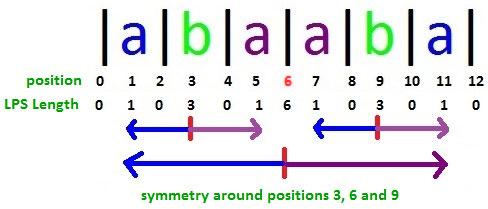
\includegraphics[width=0.7\columnwidth]{fig/ltlp1.png}
    \caption{LPS length at each position for palindrome. }
    \label{fig:ltlp}
\end{figure}
The code for Python 2 is given: and try to understand later???
\begin{lstlisting}[language = Python]
def manachers(S):
    A = '@#' + '#'.join(S) + '#$'
    Z = [0] * len(A)
    center = right = 0
    for i in xrange(1, len(A) - 1):
        if i < right:
            Z[i] = min(right - i, Z[2 * center - i])
        while A[i + Z[i] + 1] == A[i - Z[i] - 1]:
            Z[i] += 1
        if i + Z[i] > right:
            center, right = i, i + Z[i]
    return Z

return sum((v+1)/2 for v in manachers(S))
\end{lstlisting}
\item \textbf{Longest Palindromic Subsequence (L516, **).} Given a string s, find the longest palindromic subsequence's length in s. You may assume that the maximum length of s is 1000. 
\begin{lstlisting}[numbers=none]
Example 1:
Input:
"bbbab"
Output:
4
One possible longest palindromic subsequence is "bbbb".

Example 2:
Input:
"cbbd"
Output:
2
One possible longest palindromic subsequence is "bb". 
\end{lstlisting}
\textbf{Solution: Range Type Dynamic Programming.} We use dp[i][j] to denote the maximum palindromic subsequence of s(i,j). Like the substring palindrome, we only need to fill out the upper bound of the matrix. Let us dismentle the problems into different length of substring:
\begin{lstlisting}[numbers=none]
L=2: bb bb ba ab i=0..n-L+1, j=i+L-1
L=3: bbb bba bab, if s[i] == s[j], Yes: dp[i][j] = dp[i+1][j-1]+2, which we obtined from last L2, No: dp[i][j] = max(dp[i+1][j], dp[i][j-1])
L=4, bbba, bbab
L=5, bbbab
\end{lstlisting}
The process will be controled by the range of the length of substring. And we fill out the matrix in the following way: this is a ranging type of dynamic programming. 
\begin{lstlisting}[numbers=none]
[[1, 2, 0, 0, 0], [0, 1, 2, 0, 0], [0, 0, 1, 1, 0], [0, 0, 0, 1, 1], [0, 0, 0, 0, 1]]
[[1, 2, 3, 0, 0], [0, 1, 2, 2, 0], [0, 0, 1, 1, 3], [0, 0, 0, 1, 1], [0, 0, 0, 0, 1]]
[[1, 2, 3, 3, 0], [0, 1, 2, 2, 3], [0, 0, 1, 1, 3], [0, 0, 0, 1, 1], [0, 0, 0, 0, 1]]
[[1, 2, 3, 3, 4], [0, 1, 2, 2, 3], [0, 0, 1, 1, 3], [0, 0, 0, 1, 1], [0, 0, 0, 0, 1]]
\end{lstlisting}
\begin{lstlisting}[language=Python]
def longestPalindromeSubseq(self, s):
    if not s:
        return 0
    if s == s[::-1]:
        return len(s)
    
    rows = len(s)
    dp = [[0 for col in range(rows)] for row in range(rows)]
    for i in range(0,rows):
        dp[i][i] = 1
    
    for l in range(2, rows+1): #use a space
        for i in range(0,rows-l+1): #start 0, end len -l+1
            j = i+l-1
            if j > rows:
                continue
            if s[i] == s[j]:
                dp[i][j] = dp[i+1][j-1]+2
            else:
                dp[i][j] = max(dp[i][j-1], dp[i+1][j])
    return dp[0][rows-1]
\end{lstlisting}
\end{examples}
\subsection{Calculator}
In this section, for basic calculator, we have operators '+', '-', '*', '/', and parentheses. Because of ('+', '-') and ('*', '/') has different priority, and the parentheses change the priority too. The basic step is to obtain the integers digit by digit from the string. And, if the previous sign is '-', we make sure we get a negative number.  Given a string expression: (a+b/c)*(d-e)+((f-g)-(h-i))+(j-k). The rule here is to deduct this to:
\begin{equation}
    \underline{\underline{(a+\underline{b/c}_b)}_a*\underline{(d-e)}_d}_a+\underline{(\underline{(f-g)}_f-\underline{(h-i)}_h)}_f+\underline{(j-k)}_j
\end{equation}
The rules are: 1) Reduce the '*' and '/': And we handle it when we encounter the following operator or at the end of the string. Because, when we encounter a sign(operator), we check the previous sign, if the previous sign is '/' or '*', we compute the previous number with current number to reduce it into one. 2) Reduce the parentheses into one: (d-e) is reduced to d, and because the previous sign is '*', it is further combined with a and become a. Thus, if we save the reduced result into a stack, there will be [a,, f, j], we just need to sum over. thus to avoid the boundary condition, we can add '+' at the end. In the later part, we will explain more about how to deal with the above two kinds of reduce. There are different levels of calculators:
\begin{enumerate}
    \item \label{case_1}'+', '-', w/o parentheses: e.g.,  a+b+c, or a-b-c.
    \begin{lstlisting}[numbers=none]
    presign = '+', num=0,  for the digits, stack for saving either negative or positive integer
    1. iterate through the char:
        if a digit: obtain the integer
        else if c in ['+, '-'] or c is the last char:
            if presign == '-': 
                num = -num
            stack.append(num)
            num = 0
            presign = c
    2. sum over the positive and negative values in the stack
    \end{lstlisting}
    \item '+', '-',  with parentheses: e.g. a-b-c vs a-(b-c-d). To handle the parentheses, we need to think of (b-c-d) as a single integer. When we encounter the left parenthesis we save its state: the previous sign and '('; when encountering ')', we do a sum over in the stack till we pop out the previous '('. And we recover its state: the previous sign and the num. 
    \begin{lstlisting}[numbers=none]
    if c == '(':
        stack.append(presign)
        stack.append('(') 
        presign = '+'
        num = 0
    else if c in ['+, '-', ')']: # if its operator or ')'
        if presign == '-': 
                num = -num
        if c == ')':
            sum over in the stack till top is '(',
            restore the state
        else:
            stack.append(num)
            num=0, presign = c
    \end{lstlisting}
    \item '+', '-', '*', '/', w/o parentheses: This is similar to Case~\ref{case_1}, other than the '*', '-'. For example, a-b/c/d*e. When we are at c, we compute the pop the top element in the stack and compute (-b/c)=f, and append f into the stack. When we are at d, similarly, we compute (f/d)=g, and append g into the stack. 
    \begin{lstlisting}[numbers=none]
    1. iterate through the char:
        if a digit: obtain the integer
        if c in ['+, '-', '*', '/'] or c is the last char:
            if presign == '-': 
                num = -num
            # we reduce the current num with previous
            elif presign in ['*', '/']:
                num = operator(stack.pop(),presign, num)
            stack.append(num)
            num = 0
            presign = c
    2. sum over the positive and negative values in the stack
    \end{lstlisting}
    \item '+', '-', '*', '/', with parentheses. It is a combination of the previous cases, so I am not giving code here. 
\end{enumerate}
\begin{examples}[resume]
\item \textbf{Basic Calculator (L224, ***).} Implement a basic calculator to evaluate a simple expression string. The expression string may contain open ( and closing parentheses ), the plus + or minus sign -, non-negative integers and empty spaces.
\begin{lstlisting}[numbers=none]
Example 1:
Input: "1 + 1"
Output: 2

Example 2:
Input: " 2-1 + 2 "
Output: 3

Example 3:
Input: "(1+(4+5+2)-3)+(6+8)"
Output: 23
\end{lstlisting}
\textbf{Stack for Parentheses}. Suppose firstly we don't consider the parentheses, then it is linear iterating each char and handle the digits and the sign. The code are the first if and elif in the following Python code. Now, to think of the parentheses, it does affect the result: 2-(5-6). With and without parentheses give 3 and -9 for answer. When we encounter a '(', we need to reset ans and the sign, plus we need to save the previous ans and sign, at here it is (2, -). Then when we encounter a ')', we first collect the answer from last '(' to current ')'. And, we need to sum up the answer before '('. 
\begin{lstlisting}[numbers=none]
(1+(4+5+2)-3)+(6+8)
at (: stack = [0, +]
at second '(': stack = [0, +, 1 +]
at first ')': ans=11, pop out [1, +], ans = 12, +
at second ')': ans = 9, pop out [0, +], ans = 9
at third '(': ans = 9, +, stack = [9,+], reset ans = 0, sign = '+'
\end{lstlisting}
\begin{lstlisting}[language=Python]
def calculate(self, s):
    s = s + '+'
    ans = num = 0 #num is to get each number 
    sign = '+'
    stack = collections.deque()
    for c in s:
        if c.isdigit(): #get number
            num = 10*num + int(c)
        elif c in ['-','+', ')']:
            if sign == '-':
                num = -num
            if c == ')':
                while stack and stack[-1] != '(':
                    num += stack.pop()
                stack.pop()
                sign = stack.pop()
            else:
                stack.append(num)
                num = 0
                sign = c
        elif c == '(': # left parathese, put the current ans and sign in the stack
            stack.append(sign)
            stack.append('(')
            num = 0
            sign = '+'

    while stack:
        ans += stack.pop()
    return ans
\end{lstlisting}
\item \textbf{Basic Calculator III (L772, ***).} Implement a basic calculator to evaluate a simple expression string. The expression string may contain open ( and closing parentheses ), the plus + or minus sign -, \textbf{non-negative} integers and empty spaces . The expression string contains only non-negative integers, +, -, *, / operators , open ( and closing parentheses ) and empty spaces . The integer division should truncate toward zero. You may assume that the given expression is always valid. All intermediate results will be in the range of [-2147483648, 2147483647].
\begin{lstlisting}[numbers=none]
Some examples:

"1 + 1" = 2
" 6-4 / 2 " = 4
"2*(5+5*2)/3+(6/2+8)" = 21
"(2+6* 3+5- (3*14/7+2)*5)+3"=-12
\end{lstlisting}
\textbf{Solution: Case 4}
\begin{lstlisting}[language=Python]
def calculate(self, s):
    ans = num = 0
    stack = collections.deque()
    n = len(s)
    presign = '+'
    s = s+'+'
    def op(pre, op, cur):
        if op == '*':
            return pre*cur
        if op == '/':
            return -abs(pre)//cur if pre < 0 else pre//cur
    for i, c in enumerate(s):
        if c.isdigit():
            num = 10*num + int(c)
        elif c in ['+', '-', '*', '/', ')']:
            if presign == '-':
                num = -num
            elif presign in ['*','/']:
                num = op(stack.pop(),presign, num)  
            if c == ')':  # reduce to one number, and restore the state
                while stack and stack[-1] != '(':
                    num += stack.pop()
                stack.pop() # pop out '('
                presign = stack.pop()
            else:
                stack.append(num)
                num = 0
                presign = c             
        elif c == '(': #save state, and restart a new process            
            stack.append(presign)
            stack.append(c)
            presign = '+'
            num = 0

    ans = 0
    while stack:
         ans += stack.pop()
    return ans
\end{lstlisting}
\item 227. Basic Calculator II (exercise)
\end{examples}
\subsection{Others}

Possible methods: two pointers, one loop$+$two pointers
\section{Exact Matching: Sliding Window and KMP}

\paragraph{Exact Pattern Matching}
\begin{enumerate}
    \item 14. Longest Common Prefix (easy)
\end{enumerate}

%%%%%%%%%%%%%%%%%%%%%%%%%%%%%%%%%%%%%%%%%%%%%%%%%%%%%%%%%%%%%%%%%%%%%%%%%%%
%%%%% sliding window
%%%%%%%%%%%%%%%%%%%%%%%%%%%%%%%%%%%%%%%%%%%%%%%%%%%%%%%%%%%%%%%%%%%%%%%%%%
\section{Anagram Matching: Sliding Window}
\label{string_anagram}

% \section{Sliding Window for anagram or exact matching}
However, if the question is to find all anagrams of the pattern in string S.
For example: 438. Find All Anagrams in a String

Example 1:
\begin{lstlisting}
Input:
s: "cbaebabacd" p: "abc"

Output:
[0, 6]
\end{lstlisting}

Explanation:
The substring with start index = 0 is "cba", which is an anagram of "abc".
The substring with start index = 6 is "bac", which is an anagram of "abc".

Python code with sliding window:
\begin{lstlisting}[language = Python]
def findAnagrams(self, s, p):
        """
        :type s: str
        :type p: str
        :rtype: List[int]
        """
        if len(s)<len(p) or not s:
            return []
        #frequency table
        table = {}
        for c in p:
            table[c]= table.get(c,0)+1
      
        begin,end = 0,0
        r = []
        counter = len(table)
        while end<len(s):
            end_char = s[end]
            if end_char in table.keys():
                table[end_char]-=1
                if table[end_char]==0:
                    counter-=1
            
            #go to longer string, from A, AD, 
            end+=1
            
            while counter==0: #we have the same char in the window, start to trim it
                #save the best result, just to save the beigining
                if end-begin == len(p):
                    r.append(begin)
                #move the window forward
                start_char = s[begin]
                if start_char in table: #reverse the count
                    table[start_char]+=1
                    if table[start_char]==1: #only increase when it is 1
                        counter+=1
                        
                begin+=1
        return r
\end{lstlisting}

\section{Exact Matching}
\label{string_exact_matching}
\subsection{Longest Common Subsequence}



%%%%%%%%%%%%%%%%%%%%%%%%%%%%%%%%%%%%%%%%%%%%%%%%%%%%%%%%%%%%%%%%%%%%%%%%%%%
%%%%% Longest Common Substring
%%%%%%%%%%%%%%%%%%%%%%%%%%%%%%%%%%%%%%%%%%%%%%%%%%%%%%%%%%%%%%%%%%%%%%%%%%%
\section{Exercise}
\subsection{Palindrome}
\begin{Exercise}\label{Palindrome} % this gives out 2.1 exercises
        \vspace{-\baselineskip}% <-- You don't need this line of code if there's some text here
        \Question\label{valid_pa}\textbf{Valid Palindrome (L125, *).} Given a string, determine if it is a palindrome, considering only alphanumeric characters and ignoring cases. \textit{Note: For the purpose of this problem, we define empty string as valid palindrome.}
        \begin{lstlisting}[numbers=none]
        Example 1:

Input: "A man, a plan, a canal: Panama"
Output: true

Example 2:

Input: "race a car"
Output: false
        \end{lstlisting}
\Question \textbf{Longest Palindrome (L409, *).} Given a string which consists of lowercase or uppercase letters, find the length of the longest palindromes that can be built with those letters. This is case sensitive, for example "Aa" is not considered a palindrome here.
\begin{lstlisting}[numbers=none]
Example:

Input:
"abccccdd"

Output:
7

Explanation:
One longest palindrome that can be built is "dccaccd", whose length is 7.
\end{lstlisting}

        \Question\label{Palindrome_1}\textbf{Longest Palindromic Substring(L5, **).} Given a string s, find the longest palindromic substring in s. You may assume that the maximum length of s is 1000.
\begin{lstlisting}[numbers=none]
Example 1:

Input: "babad"
Output: "bab"
Note: "aba" is also a valid answer.

Example 2:

Input: "cbbd"
Output: "bb"
\end{lstlisting}
\end{Exercise}

%%%%%%%%%%%%%%%%%end of exercise%%%%%%%%
%%%%%%%%%%start of Solution%%%%%%%%
\setboolean{firstanswerofthechapter}{true}
    %\begin{multicols}{2} % multicol is to make it has two cols
        \begin{Answer}[ref={Palindrome}]
        \Question % 1
\begin{lstlisting}[language=Python]
def isPalindrome(self, s):
    """
    :type s: str
    :rtype: bool
    """
    if not s:
        return True
    i,j = 0, len(s)-1
    s = s.lower()
    while i <= j:
        bi = s[i].isalnum() 
        bj = s[j].isalnum()
        if bi and not bj:
            j -= 1
        elif bj and not bi:
            i += 1
        elif bi and bj:
            if s[i] != s[j]:
                return False
            i += 1
            j -= 1
        else:
            i += 1
            j -= 1
    return True
\end{lstlisting}
\Question
\textbf{Solution:} The maximum length is the sum of charaters that appears even times, plus one odd charater if there is one. We can use a counter to do this. 
\begin{lstlisting}[language=Python]
def longestPalindrome(self, s):
    counter = collections.Counter(s)
        
    length = 0
    bSingle = False
        
    for v in counter.values():
        if not bSingle and v % 2 == 1:
            length += 1
            bSingle = True
        if v % 2 == 0:
            length += v
    return length
\end{lstlisting}
            \Question 
\textbf{Similar to Example~\ref{l647}}

\begin{lstlisting}[language=Python]
def longestPalindrome(self, s):
    n =len(s)
    dp = [[0 for _ in range(n)] for _ in range(n)]
    res = 0
    max_str = ''
    for i in range(n-1,-1,-1):
        for j in range(i,n):               
            if j-i>2:
                dp[i][j]=(s[i]==s[j] and dp[i+1][j-1])
            else:
                dp[i][j] =(s[i]==s[j])
            if dp[i][j] and j-i+1 >len(max_str):
                max_str = s[i:j+1]
    return max_str
\end{lstlisting}
%%%%%%%%%%%%%%%%%%%end of answer
        \end{Answer}
\setboolean{firstanswerofthechapter}{false}
\end{document}